% SPDX-License-Identifier: CC-BY-SA-4.0
% Author: Matthieu Perrin
% Part: 
% Section: 
% Sub-section: 
% Frame: 

\begingroup

\begin{frame}{Moniteur}

  \vFill
  \begin{block}{Construction de synchronisation}
    \begin{itemize}
    \item Un moniteur est un objet encapsulant des données partagées.
    \item Accès aux données partagées en exclusion mutuelle.
    \item Méthodes gardées par des conditions bloquantes (gardes).
    \end{itemize}
  \end{block}

  \vFill
  \hFill
  \begin{minipage}{.4\textwidth}
    \begin{center}
      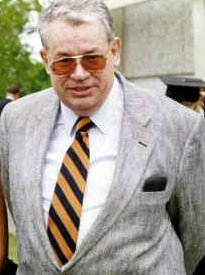
\includegraphics[height=3cm]{hansen}\\
      Per Brinch Hansen
    \end{center}
  \end{minipage}
  \hFill
  \begin{minipage}{.5\textwidth}
    \begin{center}
      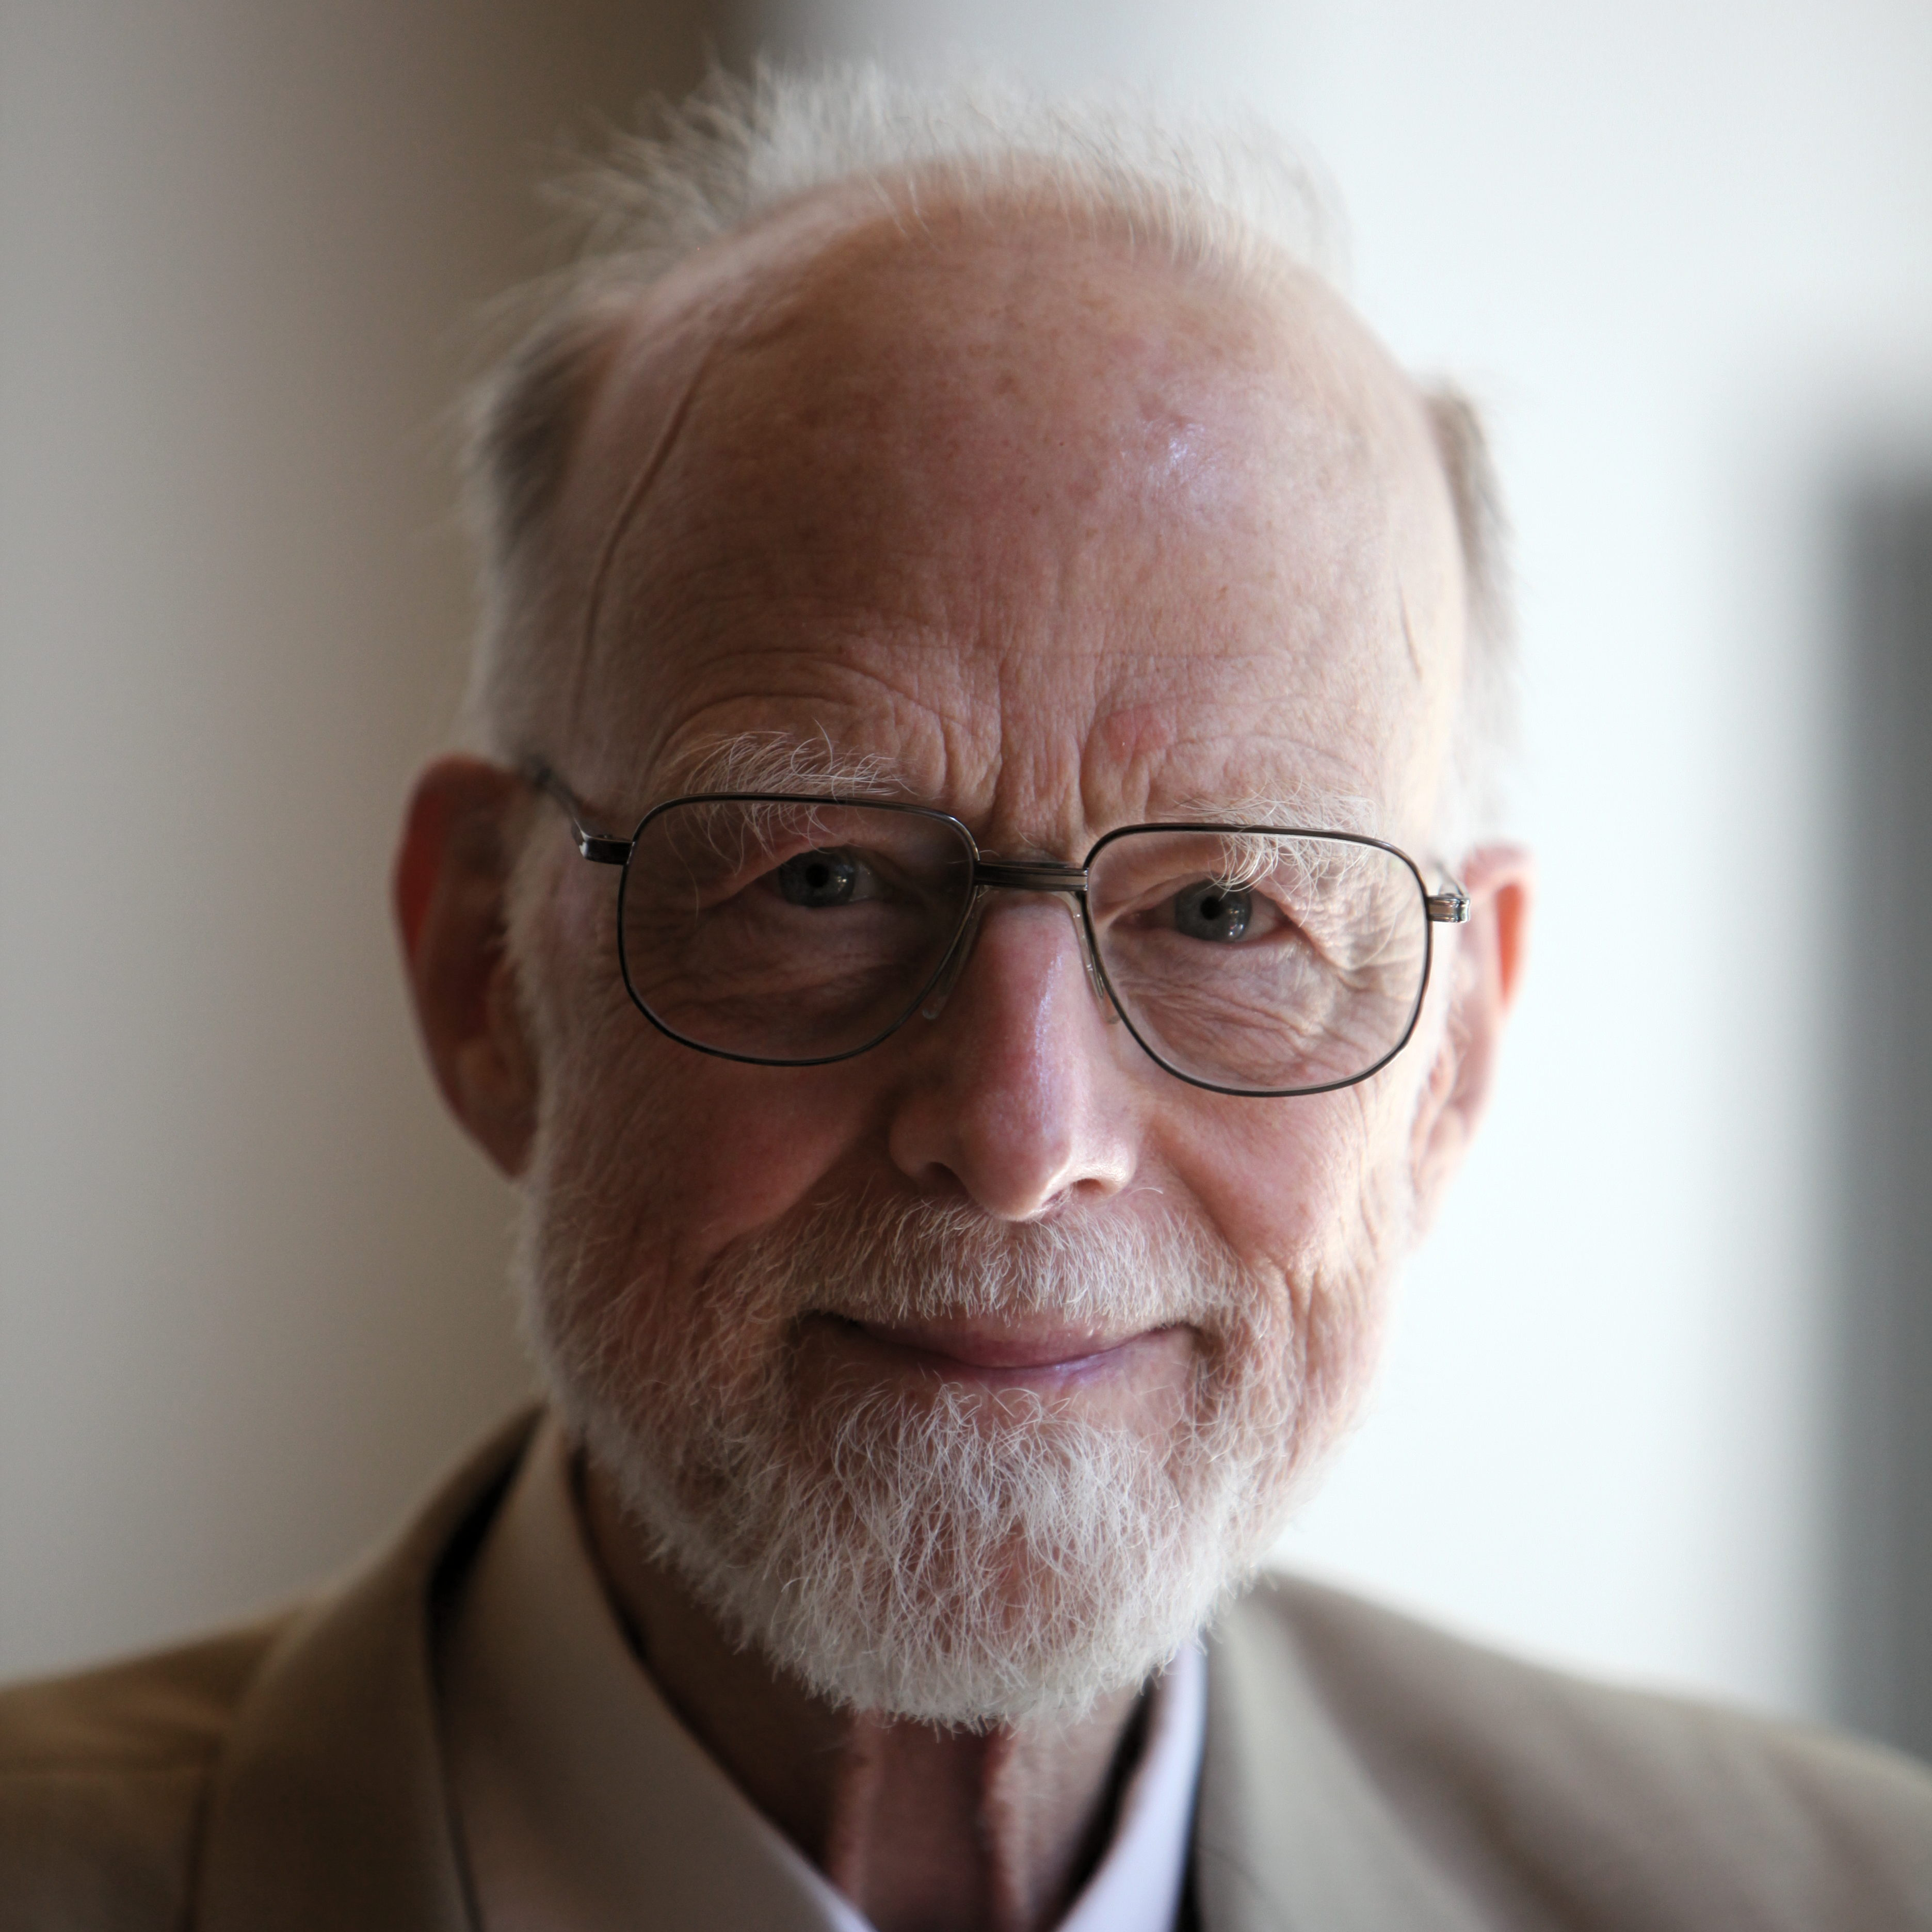
\includegraphics[height=3cm]{hoare}\\
      Tony Hoare
    \end{center}
  \end{minipage}
  \hFill

  \vFill
  \begin{citing}
  \item[] Per Brinch Hansen. \textit{Operating System Principles}. Prentice Hall (1973)
  \item[H74] C. A. R. Hoare. \textit{Monitors: an operating system structuring concept}. CACM (1974)
  \end{citing}
\end{frame}

\endgroup
\endinput
